\subsection{Decoding, held out by person}
\label{sec:decoding}

\begin{figure}[t]
\centering
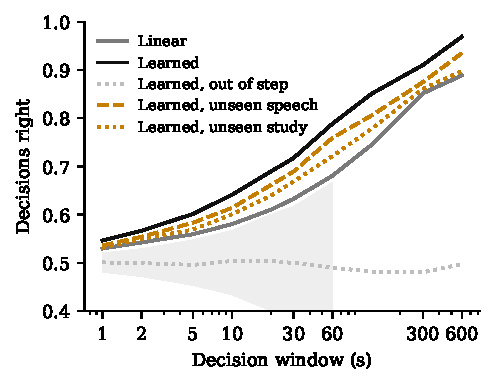
\includegraphics[width=\linewidth]{fig_windows.pdf}
\caption{Share of decisions that name the followed story against the length of EEG a decision may use, for 36 people decoded by models that never saw them: four electrodes per ear, each ear referenced to itself, no calibration. Shaded: where one person's 30 minutes cannot be told from chance (one sided binomial, 5\%). Dotted grey: the learned decoder with the speech moved 97~s out of step. Amber: one learned network per fold trained without the story content tested (dashed) or without the source study tested (dotted).}
\label{fig:windows}
\end{figure}

\begin{table}[t]
\centering
\caption{Share of decisions that name the followed story, mean over 36 held out people, four electrodes per ear, each ear referenced to itself, no calibration. Chance is 50\%. MESD: median minimal expected switch duration. Past bar: people whose one minute decisions over 30 minutes beat chance for one person (66.7\%).}
\label{tab:main}
\begin{tabular}{lrrrrrr}
\toprule
Decoder & 2~s & 10~s & 60~s & 5~min & MESD & Past bar \\
\midrule
Linear & \linTwo & \linTen & \linSixty & \linFiveMin & \linMesd~s & \linPast{} of 36 \\
Learned & \nnTwo & \nnTen & \nnSixty & \nnFiveMin & \nnMesd~s & \nnPast{} of 36 \\
Learned, out of step & & \nnCtlTen & \nnCtlSixty & & & \\
\bottomrule
\end{tabular}
\end{table}

Of the thirteen training variants compared on validation people alone, the lowest validation log loss of ten second decisions went to the base architecture trained on all five blocks per person with a learning rate of $10^{-3}$ (0.6356; a wider receptive field scored 0.6357, inside the tie margin that goes to the simpler variant; every other variant 0.6378 or more). That variant, as an ensemble of five networks per fold, names the followed story in \nnSixty{} of one minute decisions and \nnFiveMin{} of five minute ones, against \linSixty{} and \linFiveMin{} for the linear decoder (Table~\ref{tab:main}, Figure~\ref{fig:windows}), and \nnTenMin{} over ten minutes. The three random splits of the people gave \nnSplits{} at one minute. Moved 97~s out of step with the EEG, the same speech scores \nnCtlSixty{}. Every story starts at its block's first sample, so the onset of the sound could in principle carry the answer in the first window: dropping the first 10 or 30~s of every block, EEG and stories alike, left five minute accuracy at \onsetFiveTen{} and \onsetFiveThirty{} against \onsetFiveZero{} (split 7).

\subsection{Held out by story and by study}
\label{sec:heldout}

\begin{table}[t]
\centering
\caption{One network per fold (split 7), the settings of the search: what is held out besides the test people.}
\label{tab:heldout}
\begin{tabular}{lrrrr}
\toprule
Also held out & 10~s & 60~s & 5~min & Out of step, 60~s \\
\midrule
Nothing & \heldStandardTen & \heldStandardSixty & \heldStandardFiveMin & \heldStandardCtl \\
The story content tested & \heldContentTen & \heldContentSixty & \heldContentFiveMin & \heldContentCtl \\
The source study & \heldStudyTen & \heldStudySixty & \heldStudyFiveMin & \heldStudyCtl \\
\bottomrule
\end{tabular}
\end{table}

Trained without any block of the story content it was tested on, the network kept its one minute accuracy (\heldContentSixty{} against \heldStandardSixty{}) and lost a few points at five minutes; trained on one source study and tested on the other, it kept \heldStudySixty{} (Table~\ref{tab:heldout}).

\begin{table}[t]
\centering
\caption{Published one minute accuracies with electrodes around the ear, each under its own protocol, and this decoder. SS: trained on the person tested; SI: trained on other people only.}
\label{tab:lit}
\begin{tabular}{llr}
\toprule
Study & Electrodes, training & 60~s \\
\midrule
Mirkovic et al.\ \cite{mirkovic2016} & cEEGrid, 16, linked mastoids, SS & 69.3\% \\
Holtze et al.\ \cite{holtze2022} (this data set) & cEEGrid, 16, SS & 71.3\% \\
Geirnaert, Kappel, Kidmose \cite{geirnaert2025} & 19 around the ear, SS & 67.2\% \\
This work & 8, each ear referenced to itself, SI & \nnSixty \\
\bottomrule
\end{tabular}
\end{table}

\subsection{From decisions to a belief}
\label{sec:belief}

A ten second decision of the learned decoder is right \nnTen{} of the time. Fed into the belief with the fitted weight and a switch chance of 0.02 per decision, it favours the followed story after \beliefSteady{} of decisions from the second minute on. On EEG cut together from two held out listeners who followed opposite stories, the belief came over to the new story in a median of \spliceMedian~s, for \spliceFollowed{} of the switches it was in a position to follow, and favoured the followed story \spliceSteady{} of the time more than a minute after a cut.

\subsection{What holding the talker is worth}
\label{sec:hold}

Every held out person's ten second decisions were replayed under a head that sometimes looks away, by a Markov chain over three states per ten second step (facing the followed talker, facing nobody, facing the other talker, at $\pm60^\circ$), with a mean look of 20~s; the share of time looking away is an assumption and was swept. With a quarter of the time looking away, half of it at the other talker, the followed voice was the one brought forward in \holdFace{} of steps when the head alone chose (the talker faced), \holdHold{} when the last talker faced was held while facing nobody, and \holdHeadDwell{} when a new talker had to be faced for 20~s first. The belief alone gave \holdEeg{}; the phone's fusion of head and belief \holdFused{}; with the head weighed half as much ($\kappa=1$) \holdFusedKOne{}, following a real turn in a median \holdSwitchTookKOne~s; and with the head's weight growing over the first 40~s of facing a talker \holdFusedDwell{}, at a median \holdSwitchTook~s. Looking away only at nobody, the patient head rule alone reached \holdNobodyHeadDwell{}, and the belief added nothing; looking away only at the other talker, it reached \holdOtherHeadDwell{}, against \holdOtherFusedDwell{} with the dwell fusion. When attention moved and the head did not, only the belief followed: the new talker was forward in \holdCovertEeg{} of the last two minutes, against \holdCovertHeadDwell{} for the head rule, \holdCovertFused{} for the phone's fusion and \holdCovertFusedKOne{} with the head weighed half.

\subsection{In the ear and around it}
\label{sec:ear}

\begin{table}[t]
\centering
\caption{Ear-SAAD, 15 people, every person decoded by models trained on other people only, each ear referenced to itself (the scalp to its common average), causal, from the 10th second of each trial.}
\label{tab:ear}
\begin{tabular}{lrrr}
\toprule
Electrodes & Linear, 60~s & Learned, 60~s & Learned, 5~min \\
\midrule
In the ear, dry, 6 per ear & \earInLin & \earInNn & \earInNnFive \\
Around the ear, wet, 9 and 10 & \earAroundLin & \earAroundNn & \earAroundNnFive \\
Both together & \earBothLin & \earBothNn & \earBothNnFive \\
Scalp, 29 & \earScalpLin & \earScalpNn & \earScalpNnFive \\
\bottomrule
\end{tabular}
\end{table}

With dry contacts in the ear, neither decoder did better than chance; around the ear, the learned decoder reached \earAroundNn{} at one minute, and together the two sets did worse than around the ear alone (Table~\ref{tab:ear}). On the scalp, the same chain and decoders reached \earScalpNn{}. The out of step control stayed between 47\% and 51\% for every montage.

\subsection{How accuracy grows with the people trained on}
\label{sec:scaling}

Trained on $N$ people drawn from the other 35, the linear decoder's one minute accuracy rose from \scaleLinTwo{} with two to \scaleLinFifteen{} with fifteen and then stopped: \scaleLinAll{} with all 35. The learned decoder, a single network per fold trained on 5 to 25 of each fold's people and averaged over the three splits, reached \scaleNnFive{}, \scaleNnTen{}, \scaleNnFifteen{}, \scaleNnTwenty{} and \scaleNnAll{}, still rising when the folds ran out of people to train it on.

\subsection{What the electronics may add}
\label{sec:hardware}

\begin{figure}[t]
\centering
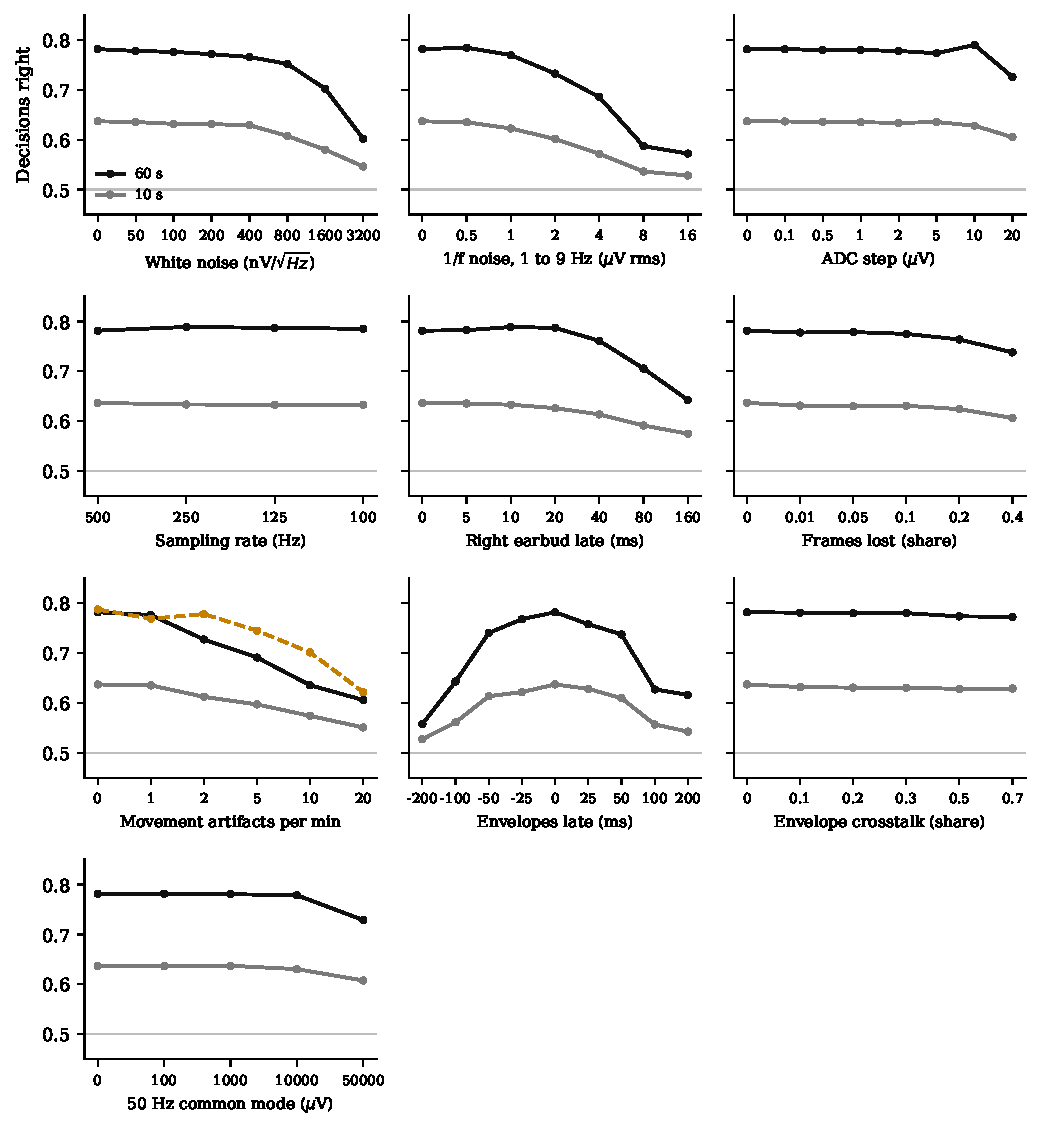
\includegraphics[width=\linewidth]{fig_hardware.pdf}
\caption{Accuracy of the final decoder (split 7, \hwNets{} networks per fold) on the raw recordings of people it never saw, degraded as an earbud's electronics might degrade them; one panel per degradation, the clean recording at its first level (at 0~ms in the envelope panel). Black: one minute decisions; grey: ten second ones; amber, dashed: one minute decisions with movement artifacts gated.}
\label{fig:hardware}
\end{figure}

Against a clean one minute accuracy of \hwNoiseBase{} with these networks (Figure~\ref{fig:hardware}), white noise added at every electrode cost less than a point up to \hwNoiseHolds{}~nV/$\sqrt{\mathrm{Hz}}$ and three points at \hwNoiseBreaks{}; 1/f noise in the decoder's band, up to \hwPinkHolds{}~$\mu$Vrms; one converter step, up to \hwLsbHolds{}~$\mu$V; and sampling, down to \hwRateHolds{}~Hz. A clock offset between the two earbuds cost nothing up to \hwSkewHolds{}~ms and three points at \hwSkewBreaks{}~ms. Frames lost one at a time cost under a point up to \hwLossHolds{} of all frames, and three points at \hwLossBreaks{}; lost in 200~ms bursts, three points at \hwBurstBreaks{}. Mains at 50~Hz, common to every electrode with 1\% imbalance, did nothing up to \hwMainsHolds{}~$\mu$V. The speech envelopes were the strictest: 25~ms late against the EEG they brought one minute accuracy to \hwEnvlagLate{}, 25~ms early to \hwEnvlagEarly{}, and three points were lost at \hwEnvlagBreaks{}~ms; the other talker mixed into each envelope, as imperfect separation would leave it, cost under a point up to \hwCrosstalkHolds{} of it.

Movement was the one degradation that cost much at a plausible rate: two 200~$\mu$V jolts a minute brought one minute accuracy to \hwArtifactsTwo{} and ten to \hwArtifactsTen{}. A gate that blanks a quarter second either side of any sample over five times its channel's spread kept \hwGatedTwo{} and \hwGatedTen{} at those rates, and on the clean recording \hwGatedClean{}: it costs nothing and belongs in the chain.


\subsection{The clench, on real recordings}
\label{sec:clench}

\begin{figure}[t]
\centering
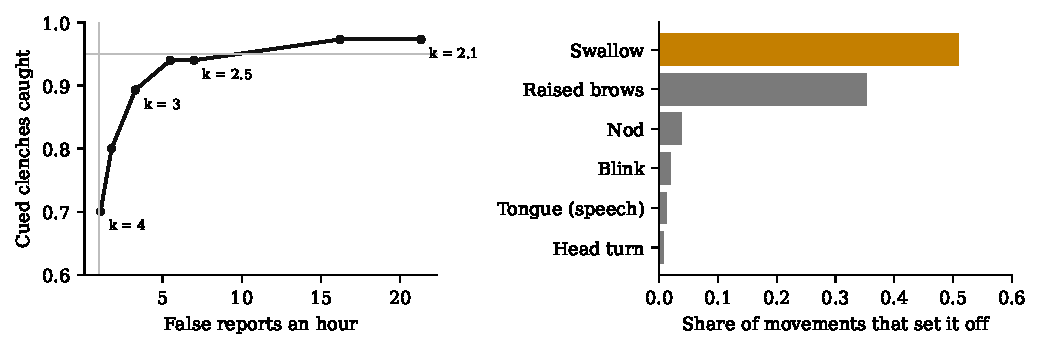
\includegraphics[width=\linewidth]{fig_clench.pdf}
\caption{The phone's clench detector, unchanged. Left: around the ear (15 people, 250~Hz), cued 3~s clenches caught against false reports an hour in blinking, eye movements, rest and heartbeat, for thresholds $k$ from 2.1 to 4 (shipped); grey lines mark the bars of 95\% caught and one false report an hour. Right: the share of each labelled movement during which it reported a gesture (12 people, temporal scalp, 1000~Hz).}
\label{fig:clench}
\end{figure}

At the shipped threshold the detector caught \clAround{} of cued clenches around the ear, \clHeadband{} on a consumer headband with one electrode behind each ear, and \clScalp{} of cued clench blocks on the temporal scalp at 1000~Hz. Around the ear the misses were concentrated: ten of fifteen people had nine or ten of their ten clenches caught, five had three or fewer, and in those five the muscle signal of the weaker ear rose only 2.4 to 3.9 times above its background during a clench, under the threshold of four. Lowering the threshold catches them and costs false reports (Figure~\ref{fig:clench}, left): \clAroundThree{} of clenches at \clAroundThreeFalse{} false an hour for $k=3$, against \clAroundFourFalse{} for $k=4$. A personal threshold set from each person's first three clenches did not reliably beat a fixed one: chosen on half the people it caught every later clench at 1.4 false an hour, and on the other half 84\% at 7.1.

Every recording without a cued clench measures false reports. In 89 minutes of rest and heartbeat around the ear there were three, in 74 minutes of blinking and eye movement none, and on the headband none at rest, six an hour while blinking and fifteen while moving the head. In \clListenHours{} hours of quiet listening (ds004015, 500~Hz, the earbud's four electrodes per ear) there were \clListen{} an hour: the median listener two, the worst 37. By labelled movement, swallowing set the detector off \clSwallow{} of the time and raised eyebrows \clBrows{}, while tongue movement as in speech did \clTongue{}, head nods and turns 0.7 to 3.8\%, blinks 1.9\% and eye movements never (Figure~\ref{fig:clench}, right).

Double clenches were the exception everywhere: \clListenDouble{} false doubles an hour in quiet listening against \clListenOthers{} singles and holds, none in the labelled movements apart from 2 of 452 tongue movements, and in every recording 20 to 50 times rarer than a false single.

Swallows could not be rejected in software. Described by what the detector could compute as it goes (the weaker ear's peak over its background, the time above half the peak, slow potentials during the event, upper against lower contacts, spectral balance and symmetry), the \clSwallowN{} labelled swallows and the \clClenchBursts{} bursts inside the cued clench blocks overlapped on every feature (the best single AUC \clSwallowBest{}), and all six together, trained on eleven people and tested on the twelfth, reached an AUC of \clSwallowAuc{}: keeping 95\% of clenches would have rejected \clSwallowKeep{} of swallows.

